\documentclass[../main.tex]{subfiles} 
\begin{document}
	A arquitetura final do processador Pires, implementada em VHDL, pode ser observada pelo RTL da figura~\ref{fig:processador_RTL}.
	
	\begin{figure}[H]
		\centering
		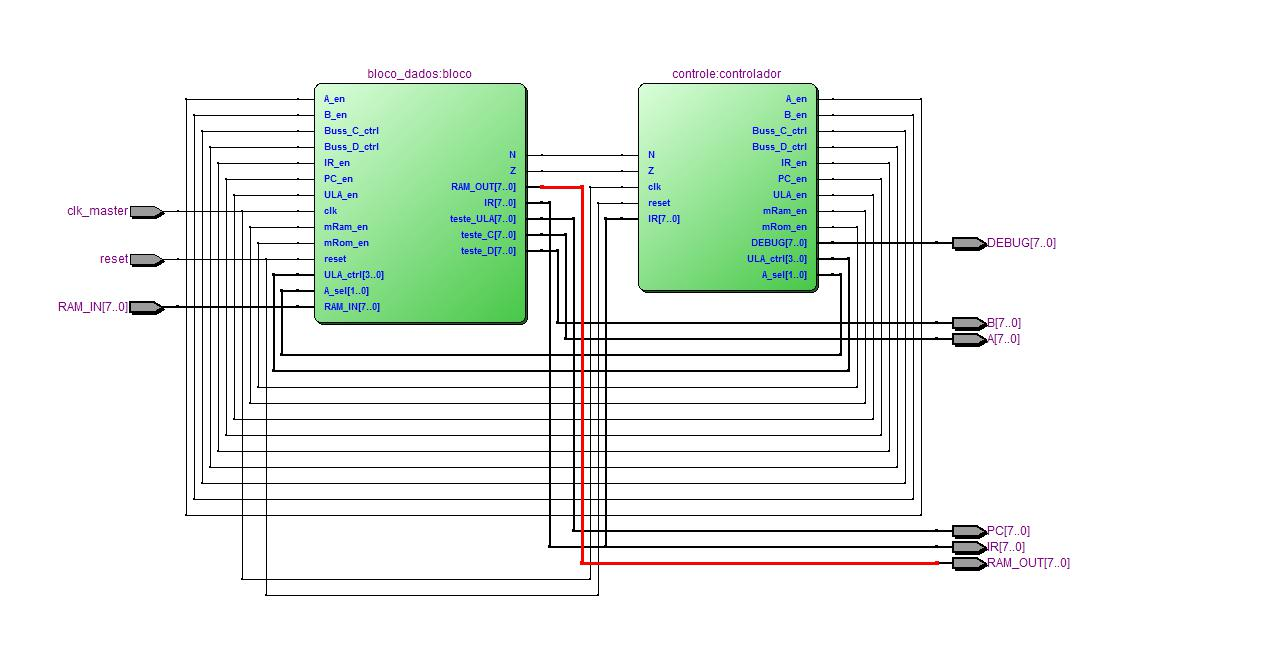
\includegraphics[width=\textwidth]{img/processador_RTL}
		\caption{Processador Pires implementado em VHDL.}
		\label{fig:processador_RTL}
	\end{figure}
	
	Esta implementação já está pronta para ser embarcada no kit de desenvolvimento baseado no FPGA \textit{Ciclone II} da \textit{Altera},
	Sendo os sinais:
	\begin{itemize}
		\item \textit{clk\_master:} Entrada de clock do processador;
		\item \textit{RAM\_OUT:} Pinos de saída ligados ao mapeamento da RAM;		
		\item \textit{RAM\_IN:} Pinos de entrada ligados ao mapeamento da RAM;
		\item \textit{reset:} Entrada de reset do processador;
		\item \textit{DEBUG:} Sinal útil na simulação, utilizado para identificar em qual estado estão as operações do processador;		
		\item \textit{A:} Sinal para simulação, mostrando o conteúdo do registrador A;		
		\item \textit{B:} Sinal para simulação, mostrando o conteúdo do registrador B;		
		\item \textit{PC:} Sinal para simulação, mostrando o conteúdo do registrador PC;		
		\item \textit{IR:} Sinal para simulação, mostrando o conteúdo do registrador IR;
	\end{itemize}
	
	A figura~\ref{fig:processador_RTL} também mostra as conexões feitas entre as entidades Bloco\_dados e Controle, implementadas
	pela entidade \textit{Top-Level} do processador. 
\end{document}